
\appendix
\chapter{Dew point measurements}\label{appendix}
The below figures show the dew point measurements for all described temperature and humidity ranges. The reference dew point is marked by the dashed blue line, the algorithmically detected dewpoint is shown by the red dashed line. The achieved dew point is correct, if the refernce dew temperature line, the detected dew temperature line and the the temperature curve intersect at the same point.

\begin{figure}[ht]
    \centering
    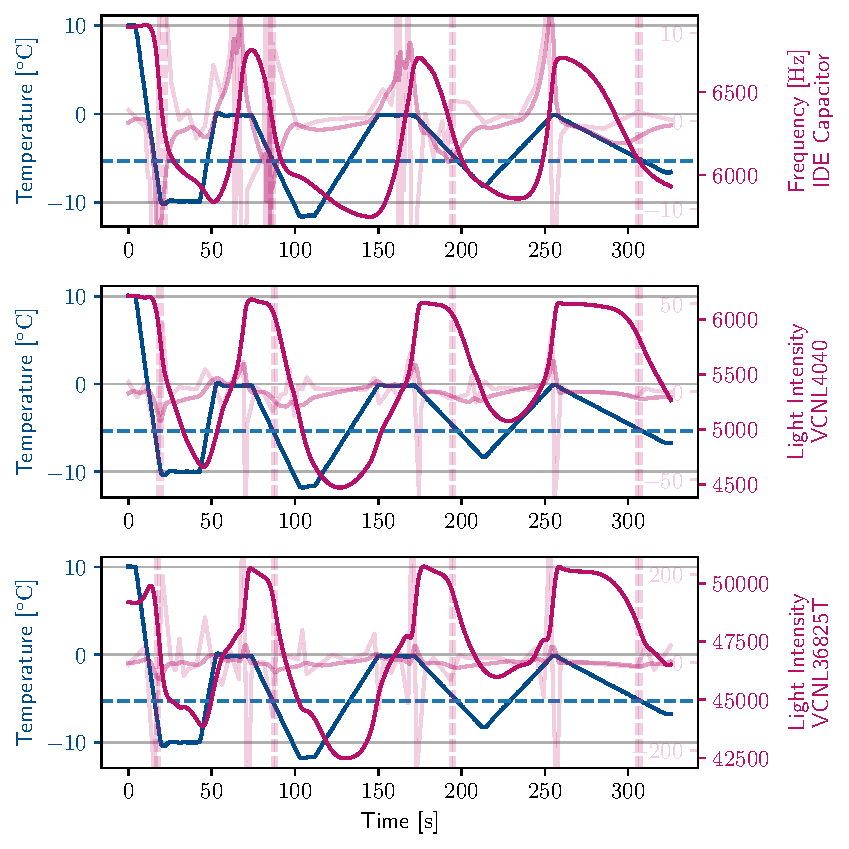
\includegraphics{graphs/t10rh33.4.pdf}
    \caption{Measurement cycle at T = \qty{10}{\celsius} and RH = \qty{33.47}{\percent}.}
    
\end{figure}

\begin{figure}[ht]
    \centering
    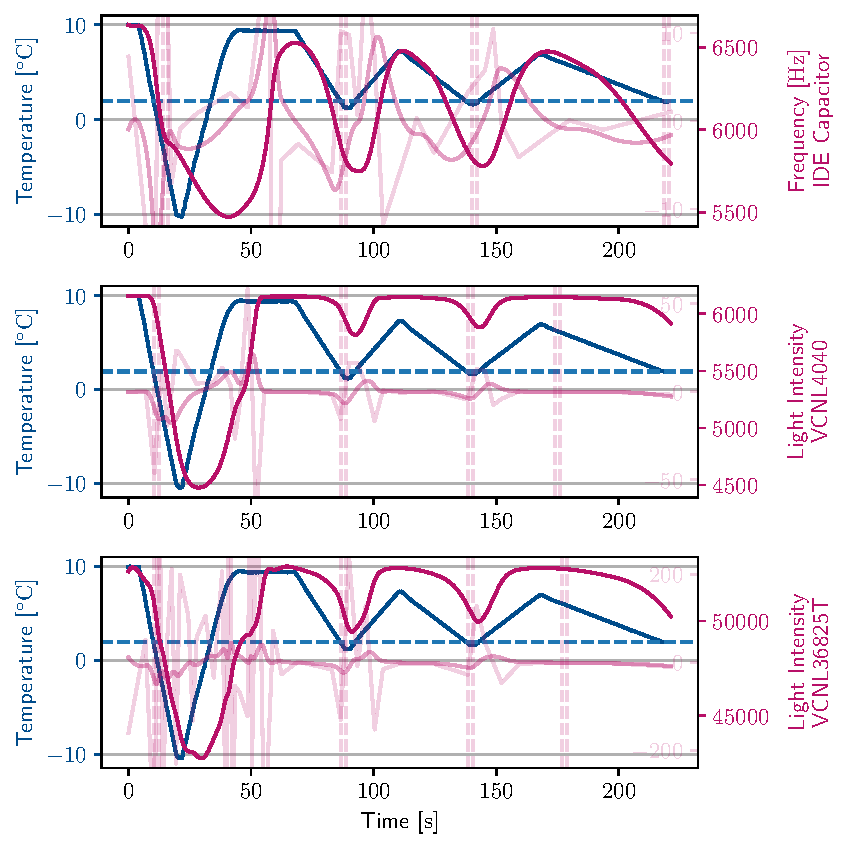
\includegraphics{graphs/t10rh57.4.pdf}
    \caption{Measurement cycle at T = \qty{10}{\celsius} and RH = \qty{57.36}{\percent}.}
    
\end{figure}

\begin{figure}[ht]
    \centering
    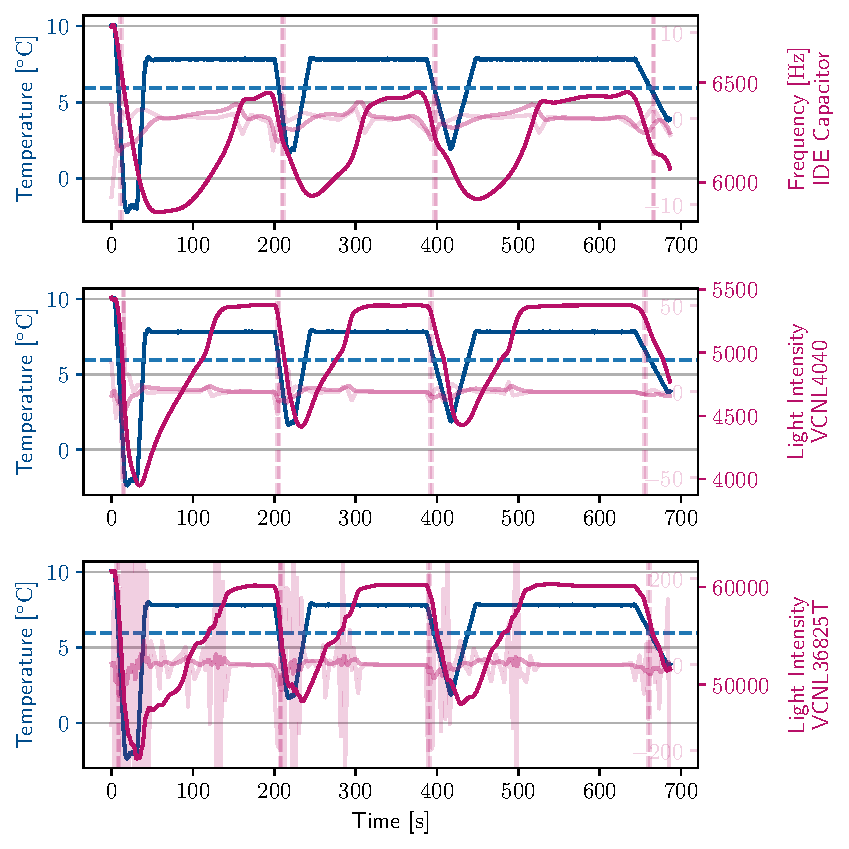
\includegraphics{graphs/t10rh75.pdf}
    \caption{Measurement cycle at T = \qty{10}{\celsius} and RH = \qty{75.67}{\percent}.}
    
\end{figure}

\begin{figure}[ht]
    \centering
    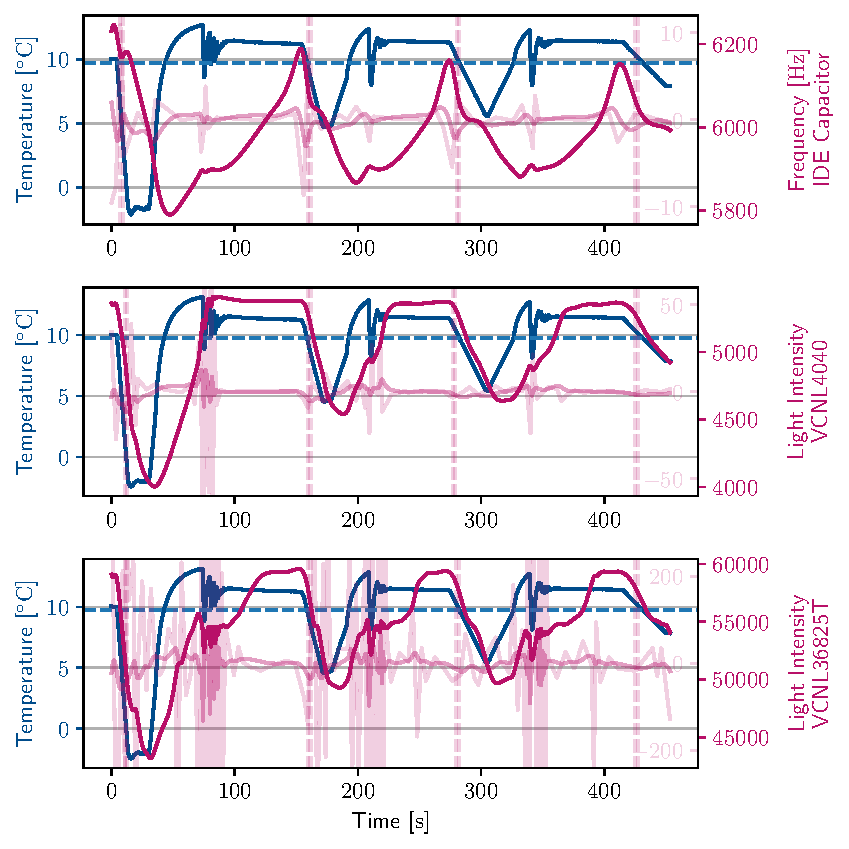
\includegraphics{graphs/t10rh98.2.pdf}
    \caption{Measurement cycle at T = \qty{10}{\celsius} and RH = \qty{98.18}{\percent}.}
    
\end{figure}

\begin{figure}[ht]
    \centering
    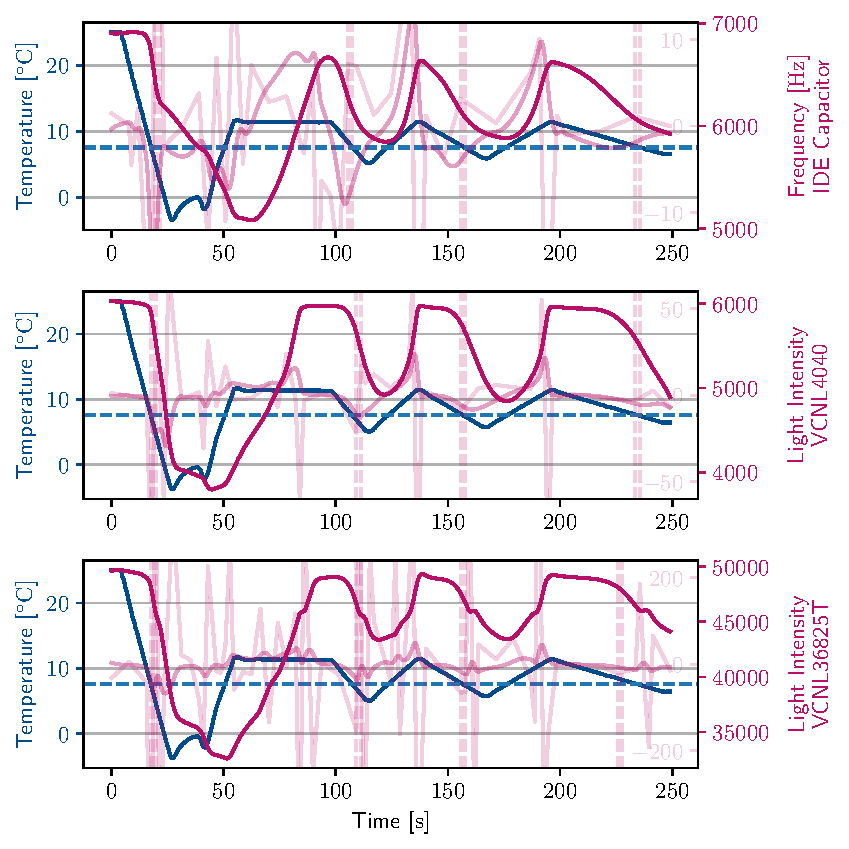
\includegraphics{graphs/t25rh32.8.pdf}
    \caption{Measurement cycle at T = \qty{25}{\celsius} and RH = \qty{32.78}{\percent}.}
    
\end{figure}

\begin{figure}[ht]
    \centering
    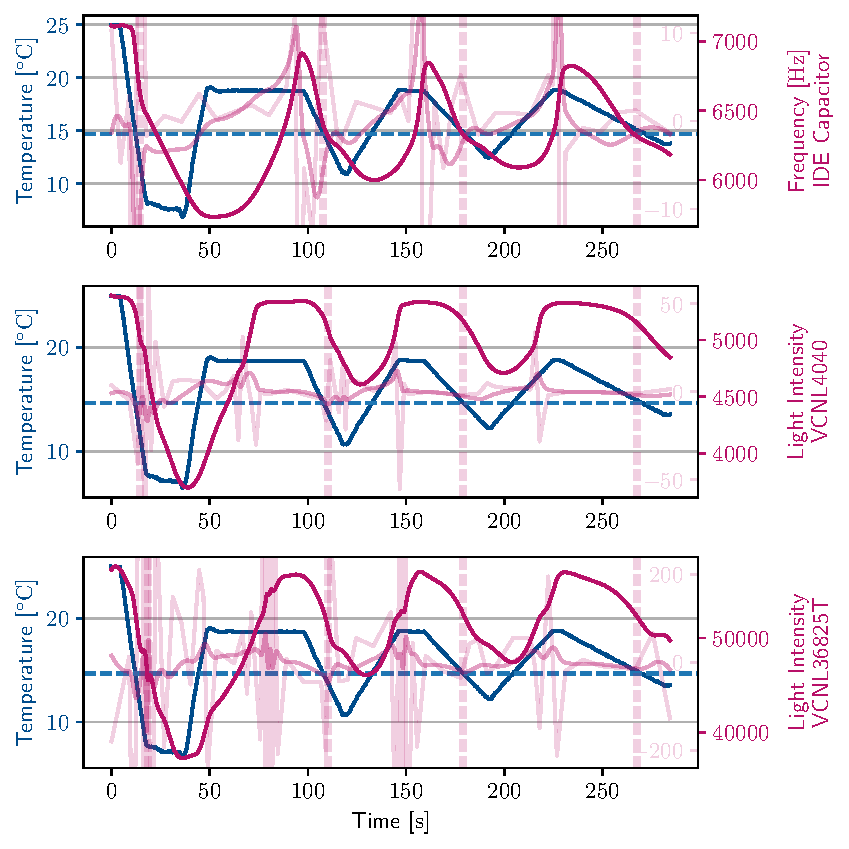
\includegraphics{graphs/t25rh52.9.pdf}
    \caption{Measurement cycle at T = \qty{25}{\celsius} and RH = \qty{52.89}{\percent}.}
    
\end{figure}

\begin{figure}[ht]
    \centering
    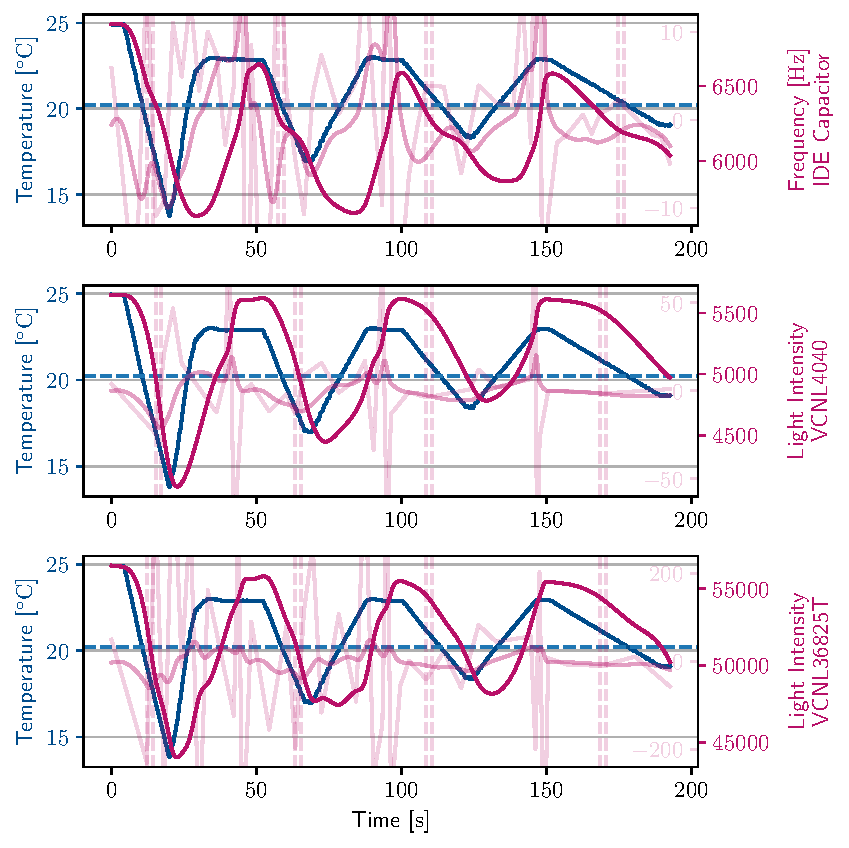
\includegraphics{graphs/t25rh75.pdf}
    \caption{Measurement cycle at T = \qty{25}{\celsius} and RH = \qty{75.29}{\percent}.}
    
\end{figure}

\begin{figure}[ht]
    \centering
    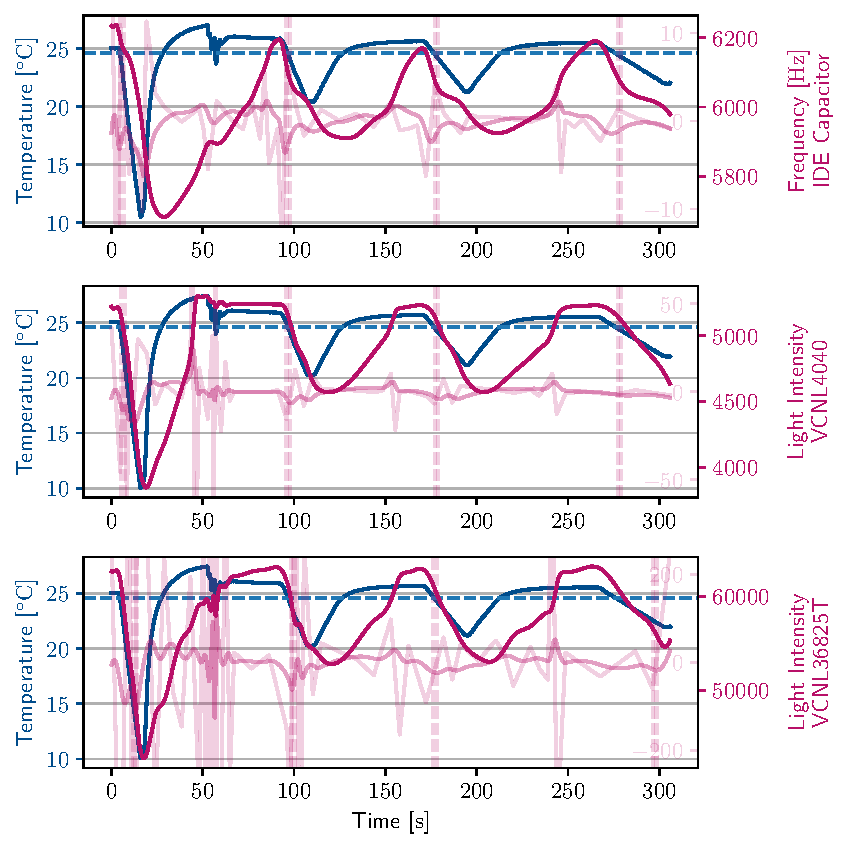
\includegraphics{graphs/t25rh97.6.pdf}
    \caption{Measurement cycle at T = \qty{25}{\celsius} and RH = \qty{97.59}{\percent}.}
    
\end{figure}

\begin{figure}[ht]
    \centering
    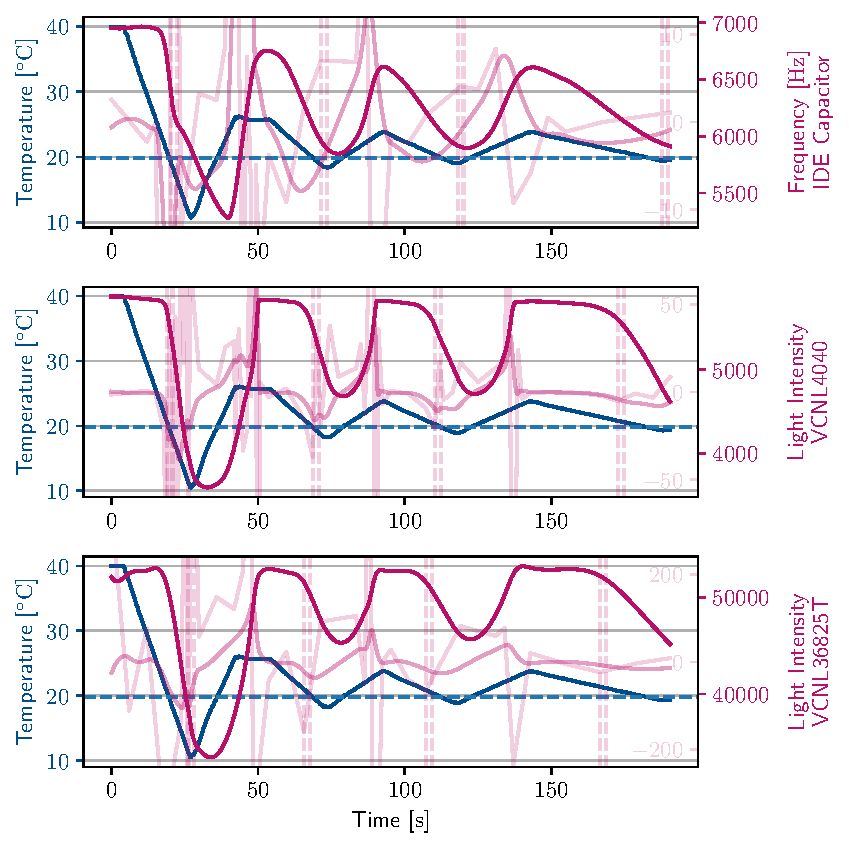
\includegraphics{graphs/t40rh31.6.pdf}
    \caption{Measurement cycle at T = \qty{10}{\celsius} and RH = \qty{31.60}{\percent}.}
    
\end{figure}

\begin{figure}[ht]
    \centering
    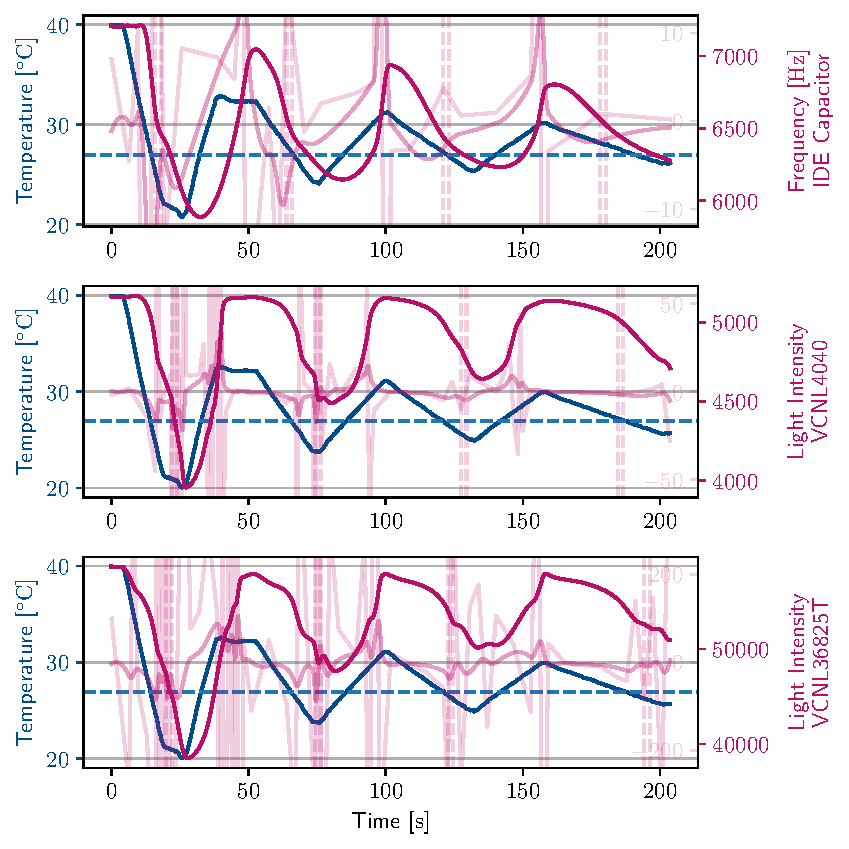
\includegraphics{graphs/t40rh48.4.pdf}
    \caption{Measurement cycle at T = \qty{25}{\celsius} and RH = \qty{48.42}{\percent}.}
    
\end{figure}

\begin{figure}[ht]
    \centering
    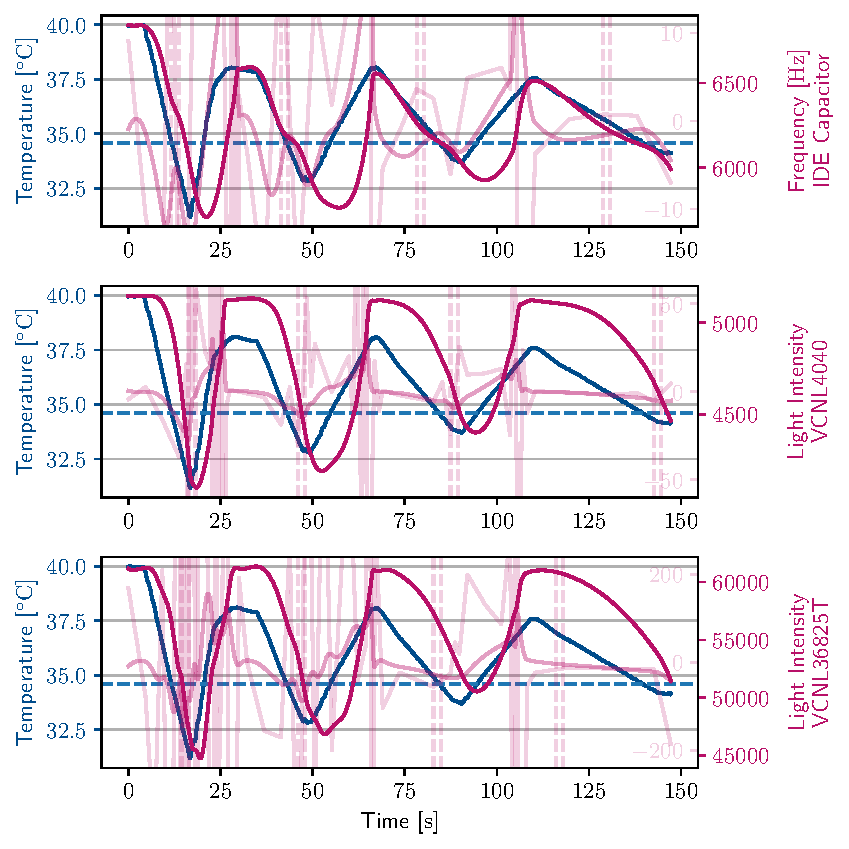
\includegraphics{graphs/t40rh75.pdf}
    \caption{Measurement cycle at T = \qty{25}{\celsius} and RH = \qty{74.68}{\percent}.}
\end{figure}

\begin{figure}[ht]
    \centering
    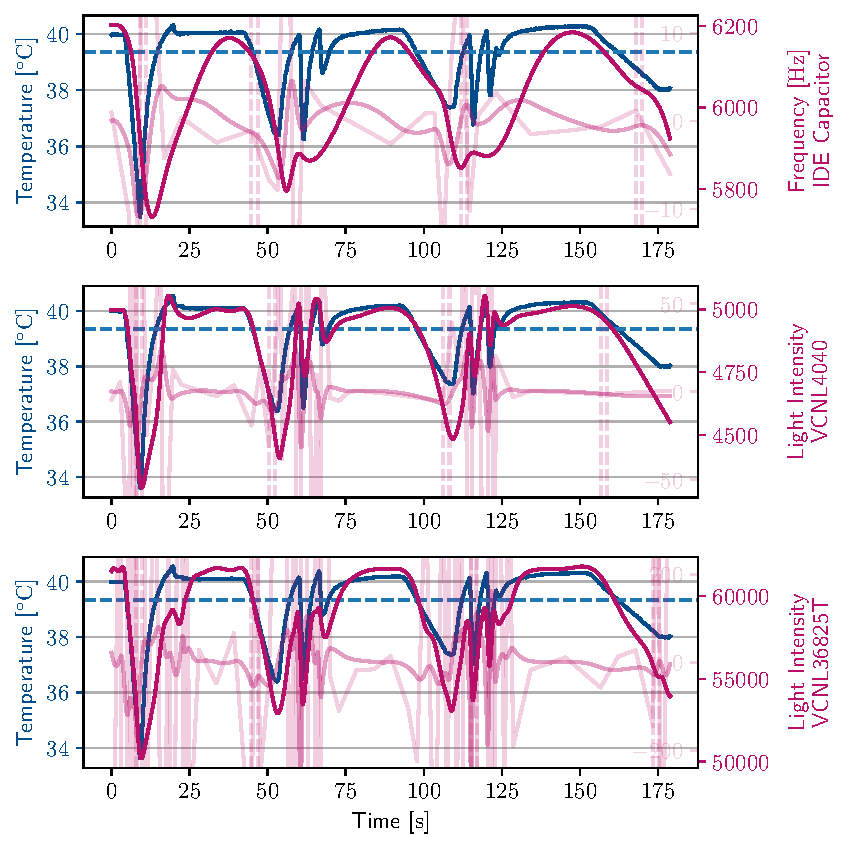
\includegraphics{graphs/t40rh96.7.pdf}
    \caption{Measurement cycle at T = \qty{25}{\celsius} and RH = \qty{96.71}{\percent}.}
\end{figure}